\documentclass[border=10pt,tikz,convert]{standalone}

% Requigray package
\usetikzlibrary{shapes, arrows.meta, positioning}
\usetikzlibrary{shadows}

\let\svtikzpicture\tikzpicture
\def\tikzpicture{\noindent\svtikzpicture}

\newlength{\w}
\setlength{\w}{4cm}

\newlength{\h}
\setlength{\h}{1.25cm}

\newlength{\s}
\setlength{\s}{3cm}

%\definecolor{outcolor}{rgb}{0.73, 0.33, 0.83}    % medium orchid
%\definecolor{incolor}{rgb}{0.85, 0.57, 0.0}			 % harvest gold
%\definecolor{hiddencolor}{rgb}{0.28, 0.82, 0.8} % medium turquoise


%\definecolor{outcolor}{rgb}{0.84, 0.32, 0.03}    % medium orchid
%\definecolor{outcolor}{rgb}{0.60, 0.37, 0.60}
%\definecolor{incolor}{rgb}{0.94, 0.63, 0.04}			 % harvest gold
%\definecolor{hiddencolor}{rgb}{0.33, 0.87, 0.88} % medium turquoise


\definecolor{outcolor}{rgb}{0.55, 0.0, 0.55}
\definecolor{hiddencolor}{rgb}{0.19, 0.55, 0.91}
\definecolor{incolor}{rgb}{0.0, 0.55, 0.55} % purple
%\definecolor{incolor}{rgb}{0.91, 0.41, 0.17} % orange

\definecolor{bgcolor}{rgb}{0.74, 0.83, 0.9}   % gray-blue



\tikzset{input/.style={draw=incolor!30, fill=incolor!30, text=incolor!20!black, minimum width=\w, minimum height=1cm,drop shadow}}
\tikzset{hidden/.style={draw=hiddencolor!30, fill=hiddencolor!30, text=hiddencolor!20!black, minimum width=\w, minimum height=1cm,drop shadow}}
\tikzset{output/.style={draw=outcolor!30, fill=outcolor!30, text=outcolor!20!black, minimum width=\w, minimum height=1cm,drop shadow}}

\begin{document}
	
	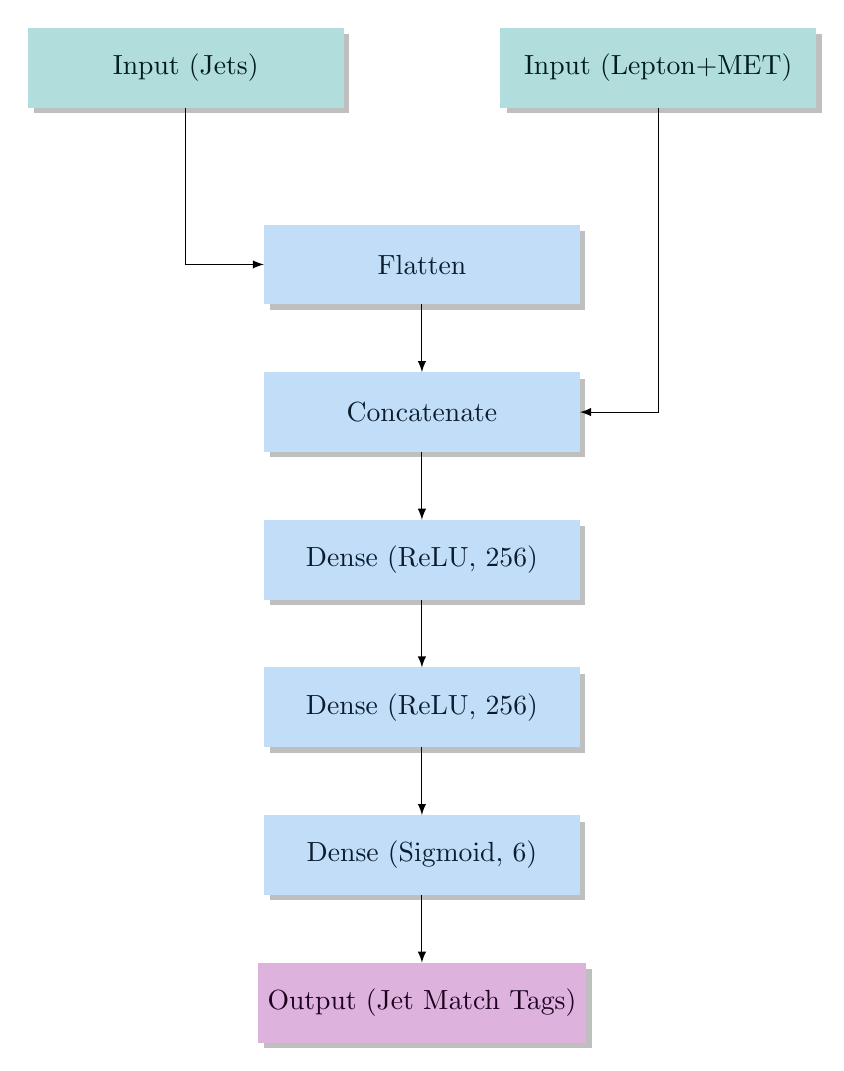
\begin{tikzpicture}
	
	%%% NODES %%%
	
	
	% INPUTS
	\node[input] at (\s,0.5*\h) (jetinput) {Input (Jets)};
	\node[input] at (3*\s,0.5*\h) (otherinput) {Input (Lepton+MET)};
	
	% JET PRETRAINER
	\node[hidden] at (2\s,-1.5*\h) (flattenedjets) {Flatten};
	\node[hidden] at (2\s,-3*\h) (concatjetsother) {Concatenate};
	\node[hidden] at (2\s,-4.5*\h) (dense256-1) {Dense (ReLU, 256)};
	\node[hidden] at (2\s,-6*\h) (dense256-2) {Dense (ReLU, 256)};
	\node[hidden] at (2\s,-7.5*\h) (jetmatchoutput) {Dense (Sigmoid, 6)};
	\node[output] at (2\s,-9*\h) (output) {Output (Jet Match Tags)};
	
	%%% ARROWS %%%
	
	% JET PRETRAINER
	\draw[-latex] (jetinput) |- (flattenedjets);
	\draw[-latex] (flattenedjets) -- (concatjetsother);
	\draw[-latex] (otherinput) |- (concatjetsother);
	\draw[-latex] (concatjetsother) -- (dense256-1);
	\draw[-latex] (dense256-1) -- (dense256-2);
	\draw[-latex] (dense256-2) -- (jetmatchoutput);
	\draw[-latex] (jetmatchoutput) -- (output);
	
	
\end{tikzpicture}
	
\end{document}


